\NeedsTeXFormat{LaTeX2e}[2005/12/01]
%%    2010/04/06 v1.0 Vorlage Master-Forschungspraktikum Versuchsauswertung
%%    based on the 2009/10/14 v0.1 GAUBM template by Prof Pruschke

\documentclass[twoside,        %% zweiseitiges Layout
               BCOR12mm,       %% Bindekorrektur 12 mm
% please comment out if report is in English
               english,ngerman, %% Dokumentspr. Deutsch, Alternativspr. Englisch
% please remove comment if report is in English 
%               ngerman,english, %% Dokumentspr. Englisch, Alternativspr. Deutsch
               fleqn,headsepline=false,footsepline=false
              ]{Vorlage/MFPREPORT}

%% Pakete und Definitionen ausgelagert
\usepackage{a4}
\usepackage{multicol}

% language option set in JGNSUM class
\usepackage{babel}
\usepackage{hyperref}

%% FONT:
%\usepackage{lmodern}
\usepackage{times} % sieht besser aus als lmodern
%\usepackage{palatino} % sieht schlechter aus als times
%\usepackage{mathpazo} % very ugly font, to be loaded later ???
%\usepackage{cmbright} % doesn't work either
\usepackage[T1]{fontenc}
\usepackage{textcomp}

\usepackage{ucs}
\usepackage[utf8x]{inputenc}

\usepackage{amsfonts}
\usepackage{amstext}
\usepackage{amsmath}
\usepackage{amsthm}
\usepackage{amssymb}
\usepackage{amsbsy}   % AMS-Boldsymbol

% \usepackage{mathabx} % e.g. for \Sun
%% but not a standard package (neither texlive nor Miktex)
%% so use wasysym (\astrosun) instead
\usepackage{wasysym} % e.g. for \astrosun or \CheckedBox

\usepackage{bbm,mathrsfs}

\usepackage{textcomp} % noch einige coole symbole

\usepackage{sectsty}
\allsectionsfont{\raggedright}

\usepackage[numbers]{natbib}
\citestyle{dinat}
\bibliographystyle{dinat}

\usepackage{makeidx}

\usepackage{url}	% für hübsche URLs mit Link
\usepackage{color}	% für farben a la \definecolor{Gray}{gray}{0.5}
\usepackage{verbatim}
\usepackage{subfigure}
\usepackage{listings}

\usepackage{fancybox}
%usage:
%\begin{Verbatim}[frame=single,label=Titel]
%Verbatim Zeile
%\end{Verbatim}


 \setlength{\textwidth}{16.2cm}
 \setlength{\textheight}{24cm}
 \setlength{\oddsidemargin}{0cm}
 \setlength{\evensidemargin}{-0.5cm}

 %unbedingt nach abmessungen einfügen!
 \usepackage{fancyhdr}
 \pagestyle{fancy}
 %\sloppy % für weniger absatzfehler

 \setcounter{tocdepth}{2}
 \setcounter{secnumdepth}{2}

 \ifreportelse{\numberwithin{equation}{chapter}}{\numberwithin{equation}{section}}
 \theoremstyle{plain}% default
 \ifreportelse{\newtheorem{thm}{Theorem}[chapter]}{\newtheorem{thm}{Theorem}[section]}

 \newtheorem{satz}{Satz}
 \newtheorem{lem}[thm]{Lemma}
 \newtheorem{prop}[thm]{Proposition}
 \newtheorem{kor}[thm]{Korollar}
 \newtheorem{cor}[thm]{Corollary}

 \theoremstyle{definition}
 \newtheorem{defi}{Definition}

 \def\@proof{%
  \if@englishpreamble{Proof}\else{Beweis}\fi
 }
 \newenvironment{bew}{\begin{proof}[\@proof]}{\end{proof}}



%% einbinden einiger nützlicher Befehle
\newcommand{\iflanggerman}[2]{
 \iflanguage{german}{#1}{
  \iflanguage{ngerman}{#1}{#2}
 }
}

% box around the whole equation, number inclusive
\newcommand{\boxedeqn}[1]{%
  \[\fbox{%
      \addtolength{\linewidth}{-2\fboxsep}%
      \addtolength{\linewidth}{-2\fboxrule}%
      \begin{minipage}{\linewidth}%
      \begin{equation}#1\end{equation}%
      \end{minipage}%
    }\]%
}

\iflanggerman{
 \newcommand{\const}{\mathrm{konst}}
 \newcommand{\Const}{\mathrm{konst.}}
}{
 \newcommand{\const}{\mathrm{const}}
 \newcommand{\Const}{\mathrm{const.}}
}

% von Meier
\newcommand{\nbd}{\nobreakdash-\hspace{0pt}}
% example: $K$\nbd{}Vektorraum
\newcommand*{\transpose}[1]{\prescript{t}{}{#1}}
\newcommand*{\conjugate}[1]{\overline{#1}}
\newcommand*{\abs}[1]{\lvert#1\rvert}
\newcommand*{\Mod}{\mathrm{mod}}
\newcommand{\symdif}{\mathbin\triangle}
\DeclareMathOperator{\Graph}{Graph}
\DeclareMathOperator{\id}{id}
\DeclareMathOperator*{\grad}{grad}
\DeclareMathOperator*{\Div}{div}
\DeclareMathOperator*{\rot}{rot}
\DeclareMathOperator{\sig}{sig}
\DeclareMathOperator{\sgn}{sgn}
\DeclareMathOperator{\diag}{diag}
\DeclareMathOperator{\tr}{tr}
\DeclareMathOperator{\Sp}{Sp}
\DeclareMathOperator{\im}{Im}
\DeclareMathOperator{\re}{Re}

\newcommand{\vcentcolon}{\mathop{:}}



%Zur Formatierung in der Matheumgebung
\renewcommand{\t}{\ensuremath{\rm\tiny}} % Tiefgestellter Text in der Matheumgebung wird schoener mit: $\Phi_{\t{Text}}$
\renewcommand{\d}{\ensuremath{\mathrm{d}}} % Die totale Ableitung ist stets aufrecht zu setzen: \d
\newcommand{\diff}[3][]{\ensuremath{\frac{\d^{#1}#2}{\d#3^{#1}}}} % einfache Ableitung nach x: $\ddx{\Phi}$
\newcommand{\pdiff}[3][]{\ensuremath{\frac{\partial^{#1}#2}{\partial#3^{#1}}}} % wie gesprochen, eine partielle Ableitung: \del
\newcommand{\aeqiv}{\ensuremath{\qquad \Longleftrightarrow \qquad}} % Eine Aequivalenz
\newcommand{\folgt}{\ensuremath{\qquad \Longrightarrow \qquad}} % Ein Folgepfeil mit Abstaenden
\newcommand{\corresponds}{\ensuremath{\mathrel{\widehat{=}}}} % Befehl für "Entspricht"-Zeichen
\newcommand{\mi}[1]{\ensuremath{\mathit{#1}}} % italics für griechische Buchstaben in Matheumgebung

%Um nicht so viel schreiben zu müssen...
\newcommand{\bs}[1]{\boldsymbol{#1}}
\newcommand{\ol}[1]{\overline{#1}}
\newcommand{\wtilde}[1]{\widetilde{#1}}
\newcommand{\mrm}[1]{\mathrm{#1}}
\newcommand{\mbf}[1]{\mathbf{#1}}
\newcommand{\mbb}[1]{\mathbb{#1}}
\newcommand{\mcal}[1]{\mathcal{#1}}
\newcommand{\mfrak}[1]{\mathfrak{#1}}

%Abkürzungen
\newcommand{\zB}{z.\,B.\ }
\newcommand{\bzw}{b.\,z.\, w.\ }
\newcommand{\Dh}{d.\,h.\ }
\newcommand{\Gl}{Gl.\ }
\newcommand{\Abb}{Abb.\ }
\newcommand{\Tab}{Tab.\ }


\begin{document}
\LabratoryName{FM.TES}{Tunneleffekt bei Supraleitern}
\ProtocolAuthor{Eric}{Bertok}{eric.bertok@stud.uni-goettingen.de}
\Assistant{Christoph}{Meyer}
\ResearchFocus{Festkörper- und Materialphysik (M.phy.403)}
% In der naechsten Version beruecksichtigt
%\Collaborator{Vorname}{Nachname}{email}
\ConductedOn{25}{2}{2017}
\date{\today}
% eines von beiden
\CopyNotWanted
%\CopyWanted

\pagenumbering{roman}
\maketitle

%\begin{otherlanguage}{english}
%\end{otherlanguage}

\tableofcontents

\clearpage
\pagenumbering{arabic}

\section{Einleitung}
\label{sec:einleitung}
Supraleiter sind elektrische Leiter, die unterhalb einer bestimmten Temperatur,
genannt kritische Temperatur, einen Elektrischen Widerstand von Null haben.
Dies ist von immenser Bedeutung , zum Beispiel für die Herstellung von starken Magnetfeldern
und verlustfreien Stromleitungen. Aber auch für Grundlagenforschung sind
Supraleiter relevant. Sie sind das Beispiel eines sogenannten makroskopischen
Quanteneffektes, bei der alle Elektronen sich im exakt gleichen Quantenzustand
befinden. Eine Untersuchung von den Eigenschaften der Supraleiter erlaubt also
Einblicke in die Quantentheorie, insbesondere die Vielteilchendynamik von
Elektronen und die Gitterdynamik der Festkörper.
Eine besonders geeignete Herangehensweise für die Untersuchung von Supraleitern
ist die Ausnutzung des Tunneleffektes, ein weiterer quantenmechanischer Effekt.
Durch ihn lassen sich direkt eine Vielzahl an qualitativen und quantitativen
Eigenschaften von Supraleitern erschließen, insbesondere die Zustandsdichte
(siehe Unten).\\
In diesem Versuch soll zunächst ein Aluminium-Aluminiumoxid-Blei Tunnelkontakt
hergestellt und anschließend auf Supraleitung untersucht werden. Dabei werden
außerdem eine grundlegende experimentelle Methode der Tieftemperaturphysik,
nämlich das Abkühlen der Messsonde auf wenige Grad Kelvin geübt.
Die gemessenen Daten werden anschließend auf qualitative und quantitative Art
und Weise mit Literaturwerten und der einfachsten Theorie für Supraleiter, der
BCS-Theorie, verglichen.
\section{Theorie}
\label{sec:theorie}
\subsection{Grundlagen: Zustandsdichte, Fermiverteilung, Besetzungsdichte}
Die Zustandsdichte $D(E)$ gibt die Anzahl der erlaubten Mikrozustände pro
Energieintervall $\d E$ an. Sie ist für kontinuierliche Energien allgemein
definiert durch $D(E):=\int \frac{\d^d k}{(2
\pi)^d}\delta\left(E-E(\vec{k})\right)$ \cite{hunklingerfk},
wobei $\vec k$ die Wellenzahl und $d$ die Dimension (für unseren Fall 3) ist.
$E(\vec k)$ ist die Dispersionsrelation der Teilchen.
Für freie Elektronen ergibt sich [S.\;267]\cite{hunklingerfk}:
\begin{equation}
    \label{eq:freielek}
   D_N(E_{\vec{k}})=\frac{\left(2m^*\right)^\frac{3}{2}}{2\pi ^2\hbar ^3}\sqrt{E}, 
\end{equation}
wobei $m^*$ die sogenannte effektive Masse der Elektronen ist. Diese ist für freie
Elektronen gleich ihrer tatsächlichen Masse, berücksichtigt bei einem
Festkörper aber zusätzlich den Einfluss des Kristallpotentials.

Die Fermi-Dirac Verteilung gibt die mittlere thermische Energiebesetzung von Spin-1/2
Teilchen in Abhängigkeit der Temperatur $T$ und des chemischen Potentials $\mu$
an. Sie lautet $f_T(E)=\frac{1}{\exp{\beta(E-\mu)-1}}$, wobei
$\beta=\frac{1}{k_b T}$ der Boltzmann- Faktor ist. Für $T=0$ ist sie eine
Stufenfunktion: Unterhalb der sogenannten Fermienergie $E_F=\mu$ sind alle
Zustände mit Wahrscheinlichkeit 1 besetzt, während alle oberhalb von $E_F$
unbesetzt sind. Dies bezeichnet man als ``Fermikante''.

Die Besetzungsdichte, also die Dichte der tatsächlich besetzten Zustände pro
Energieintervall erhält man als
Produkt aus Zustandsdichte und Fermiverteilung: $n(E)=D(E)f_T(E)$. Hierdurch
erreicht man eine Trennung der systemabhängigen Größen in $D(E)$ und der
systemunabhängigen Thermodynamik in $f_T(E)$.

\subsection{Tunneleffekt}
Der Tunneleffekt ist ein quantenmechanischer Effekt, bei dem ein Teilchen eine
Potentialbarriere endlicher Höhe und Breite durchqueren kann, obwohl sie höher
als die Energie des Teilchens ist. Dies kommt dadurch zustande, dass die
Wellenfunktion jenseits der Barriere verschieden von Null ist. 
Durch Lösen der Schrödingergleichung mit einer Kastenbarriere erhält man,
dass die Tunnelwahrscheinlichkeit exponentiell mit der Breite $d$ der Barriere
abfällt: \cite{giaever1961study}
\begin{align}
    \label{eq:tunnelamp}
    A_\text{tunnel}\propto e^{-\sqrt{(2m/\hbar^2 (V_0-E)}}e^{-d}.
\end{align}
Jenseits der Barriere das Potential wieder Null. Somit ist die Wellenlänge und damit die Energie des getunnelten
Teilchens unverändert. Lediglich die Wahrscheinlichkeit des Tunnelns nimmt ab.
In unserem Versuch, in dem ein Aluminium- Aluminiumoxid- Blei- Kontakt
verwendet wird, ist die Potentialbreite durch die Dicke der
Aluminiumoxidschicht gegeben. Die Höhe des Potentialwalls ist gegeben durch die
Differenz der Fermienergien der beiden Leiter Al und Pb und der des
Aluminiumoxids.
Weiterhin ist zu beachten, dass ein Teilchen nur dann durch die Barriere
tunneln kann, wenn es auf der anderen Seite freie Zustände vorfindet. Ist dies
nicht der Fall, kommt es zur exponentiellen Abnahme der Amplitude. Auf diese
Weise kann man Schlüsse über die Zustandsdichte der betrachteten Materialien
ziehen, was in diesem Versuch benutzt wird, um die Energielücke von
Supraleitern zu vermessen.

\subsection{mikroskopische Theorie der Supraleitung: Cooper- Paare}
\begin{figure}[]
    \begin{center}
        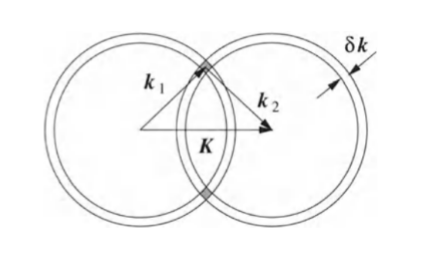
\includegraphics[scale=0.7]{fig/kreis.png}
    \end{center}
    \caption{eq: Impulsschalen im k-Raum. Impulserhaltung wird erfüllt für den
    Überlapp der beiden Schalen \cite[S.\;309]{enss2011tieftemperaturphysik}.}
    \label{fig:kreis}
\end{figure}
Die BCS Theorie, welche 1957 von Badeen, Cooper und Schrieffer entwickelt
wurde, war die erste erfolgreiche mikroskopische Theorie der Supraleitung
\cite[Kap.\;2]{buckel2013supraleitung}. Die positiven Atomrümpfe werden durch die
negativ geladenen Elektronen polarisiert. Da die Atomrümpfe vergleichsweise
schwer sind, haben sie eine geringe Schwingungsfrequenz. Dadurch kommt es zu
einer retardierten Polarisierung. Ein anderes Elektron spürt diese
Polarisierung also, wenn das erste bereits eine große Distanz zurückgelegt hat.
Aufgrund dessen kann man die Coulombabstoßung zwischen diesen beiden Elektronen
vernachlässigen. Mathematisch lässt sich diese anziehende Wechselwirkung
zwischen zwei Elektronen als ein Austausch eines virtuellen Phonons
beschreiben. Für eine detaillierte Ausarbeitung im Formalismus der zweiten
Quantisierung siehe \zB \cite[Kap.\;10.4]{enss2011tieftemperaturphysik}.
Wenn $\vec q$ der Impuls des Phonons und $\vec k_1$, $\vec k_2$ die der beiden Elektronen
sind, so gilt nach dem Austausch des Phonons
\cite[S.\;308]{enss2011tieftemperaturphysik}
\begin{align}
    \label{eq:phononimp}
    \vec k_1'=\vec k_1 +\vec q, \quad \vec k_2'=\vec k_2 -\vec q,
\end{align}
der Gesamtimpuls $\vec K=\vec k_1 + \vec k_2$ bleibt also erhalten.
Aufgrund der Fermiverteilung sind für die Elektronen nur Energien oberhalb der
Fermikante zugänglich. Approximiert man die Phononenfrequenz mit der
Debyefrequenz $\omega_D$ \cite[S\;211\;ff.]{hunklingerfk}, so liegen die freien Zustände innerhalb der
Energieschale $[E_F,E_F+\hbar \omega_D]$ oder äquivalent im k-Raum innerhalb
der Schale mit Dicke $\frac{m\omega_D}{\hbar k_F}$, wobei $k_F$ der
Fermiwellenvektor ist. Für beide Elektronen sind diese Schalen in Abb.
\ref{fig:kreis} zu sehen. Impulserhaltung ist erfüllt für alle Vektoren im
Überlapp beider Schalen. Dieser ist maximal für $\vec k_1 = -\vec k_2$. Das
Fermi Prinzip verlangt außerdem, dass beide Elektronen entgegengesetzten Spin
besitzen. Das Paar ${\vec k,\uparrow},{-\vec k,\downarrow}$ bezeichnet man als
Cooper-Paar (CP). Cooper-Paare sind effektive Bosonen. Durch die Attraktion von
Elektronenpaaren wird die Gesamtenergie verringert. Es kommt zu einer
makroskopischen Besetzung, bei der im Grundzustand alle Cooper-Paare im exakt gleichen
Quantenzustand sind \cite[Kap. 2.2]{buckel2013supraleitung}. Die Gesamtheit
aller Cooper-Paare wird deswegen als eine makroskopische Wellenfunktion
beschrieben.
\subsection{Grundzustand und Quasiteilchenanregungen}
Der im vorherigen Abschnitt beschriebene makroskopische Zustand aus
Cooper-Paaren bildet aufgrund der attraktiven Wechselwirkung den neuen
Grundzustand. Möchte man den Supraleiter in einen angeregten Energiezustand
bringen, so muss man zuerst eine Energie $\Delta$ aufbringen, um ein CP
aufzubrechen. Anschließend muss das freie Elektron auf ein höheres
Energieniveau gebracht werden, was wiederum eine Energie von $\Delta$ benötigt
\cite{tidecks1990current}. $\Delta$ Ist die Energielücke des Supraleiters,
welche hier gemessen werden soll. Die Elektronen, die bei der Aufbrechung eines CP's
entstehen, sind keine freien Elektronen, sondern Anregungungen im
Mehrelektronensystem, sogenannte Quasiteilchen. Mit Quasiteilchen können
komplizierte Mehrteilchenphänomene als Einteilchenphänomene beschrieben werden.
Aus der BCS-Theorie erhält man durch Aufstellen der freien Energie
$F=E_\text{kin}+E_\text{pot}-TS$ und deren Minimierung Ausdrücke für die
für die Anregungsenergie $E_{\vec{k}}$ der Quasiteilchenanregungen und für die
Zustandsdichte von Supraleitern $D_S(E_{\vec{k}})$ in Abhängigkeit der Energielücke: \cite[Kap.\;10.4]{enss2011tieftemperaturphysik}:

\begin{align}
    \label{eq:BCS}
    E_{\vec k}&=\sqrt{\eta_{\vec{k}}^2+\Delta^2}\\
    D_S(E_{\vec{k}})&=D_N(E_{\vec{k}})\frac{|E_{\vec k}|}{\sqrt{E_{\vec
    k}^2-\Delta^2}},\quad |E_{\vec k}|\geq\Delta_{T=0}.
\end{align}
$\eta_{\vec k}$ ist die kinetische Energie der Elektronen gemessen von der
Fermienergie. Die Quasiteilchen verhalten sich je nach kinetischer Energie wie
Löcher, Elektronen oder Mischzustände. Für $T=T_c$ ist die kinetische Energie
der Cooper-Paare groß genug, um diese aufzubrechen und der Supraleiter geht in den
normalleitenden Zustand ohne Energielücke über.

\subsection{Tunnelkennlinien von Normalleitern und Supraleitern}
\begin{figure}[]
    \begin{center}
        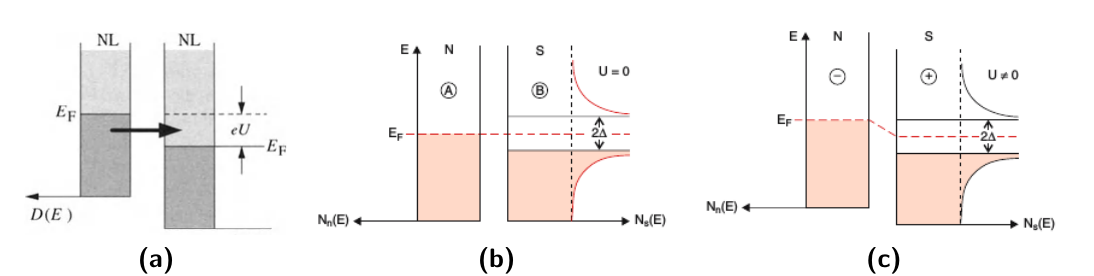
\includegraphics[width=\textwidth]{fig/tunnel.png}
    \end{center}
    \caption{Tunneleffekt zwischen zwei Normalleitern (a), zwischen einem
    Normalleiter und einem Supraleiter bei $V=0$ (b) und zwischen einem
    Normalleiter uns Supraleiter bei $U=U_c=\Delta/e$ \cite{dem}
   .}
    \label{fig:tunnel}
\end{figure}
Im Versuch werden sowohl ein Normalleiter-Normalleiter (NL/NL) und ein
Normalleiter-Supraleiterkontakt (NL/SL) verwendet. Die Situation eines NL/NL
Kontaktes ist in Abb. \ref{fig:tunnel} (a) zu sehen. Die Zustandsdichte eines
Normalleiters kann in der nähe der Fermienergie als konstant angenommen werden.
Liegt keine Spannung an, so tunneln im Mittel gleich viele Elektronen von links
nach rechts und umgekehrt. Der Strom ist null. Bei Anlegen einer Spannung
verschiebt sich das chemische Potential und Elektronen tunneln in Richtung
niedrigeren chemischen Potentials in die zugänglichen freien Zustände.
Man erwartet eine Proportionalität zwischen der anliegenden Spannung und dem
gemessenen Tunnelstrom, also Ohm'sches verhalten $U=RI$.
Für einen NL/SL Kontakt liegt die Fermienergie des Normalleiters in der Mitte
der Energielücke des Supraleiters. Somit kann kein Tunnelstrom fließen, da
keine freien Zustände unterhalb $E_F$ vorhanden sind (\ref{fig:tunnel} (b) ). Erst bei einer Spannung
\begin{figure}[]
    \begin{center}
        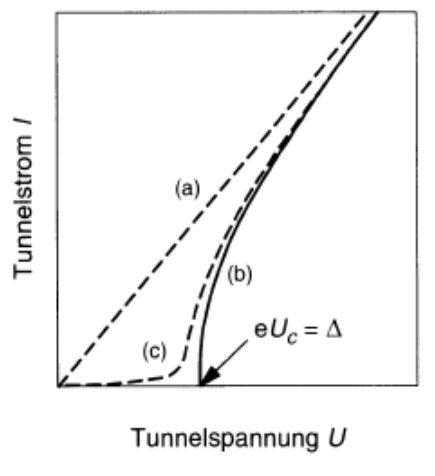
\includegraphics[scale=0.5]{fig/kennlinie.png}
    \end{center}
    \caption{Tunnelkennlinie eines NL/NL Kontaktes (a), eines NL/SL Kontaktes
    bei $T=0$ (b) und eines NL/SL Kontaktes bei $0<T<T_c$ (c) \cite[S:\;72]{buckel2013supraleitung}.}
    \label{fig:kennlinie}
\end{figure}
von $U=\Delta/e$ können Elektronen in den Supraleiter Tunneln und man misst
einen Tunnelstrom. Dieser steigt sehr steil an, da die Zustandsdichte des
Supraleiters eine Van Hove-Singularität aufweist \cite[S\;209]{hunklingerfk} (\ref{fig:tunnel} (c) ).
Die Tunnelstrom- Kennlinien sind in Abb. \ref{fig:tunnel} für die verschiedenen
Fälle gezeigt. Für $T\neq 0$ ist die Energielücke kleiner als bei $T=0$.
Außerdem können durch thermische Fluktuationen bereits früher Elektronen in den
Supraleiter tunneln. Dies führt zu einer Aufweichung der Kennlinie
(\ref{fig:kennlinie} (c) ).


\section{Durchführung}
\label{sec:durchfuehrung}
\subsection{Herstellung der Probe}
\begin{figure}[]
    \centering
    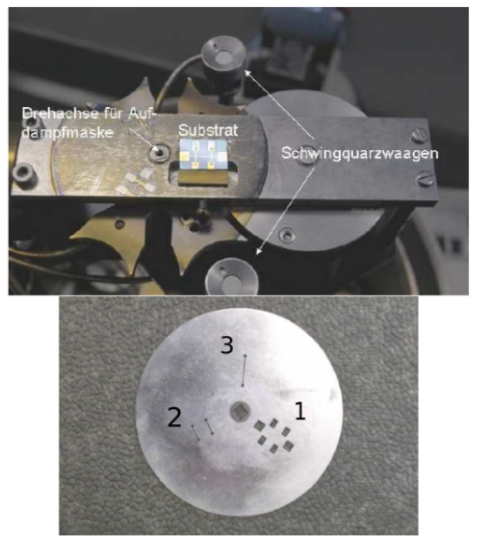
\includegraphics[scale=0.5]{fig/aufbau.png}
    \caption{Versuchsaufbau zur Herstellung der Probe. Oben: Substrathalter und
        Schwingungsquarzwaagen.
        Unten: Drehblende \cite{fprakt}.}
    \label{fig:aufbau}
\end{figure}
Zunächst wird die Probe hergestellt. Dazu wird ein SiO$_2$-Wafer verwendet,
auf den die Tunnekontakte draufgedampft werden. Dieser wird zunächst in die
Halterung der Vakuumglocke eingespannt. Jetzt muss die Schablone für das
Aufdampfen montiert werden, wobei auf die korrekte Orientierung zu achten ist.
Desweiteren muss das gesamte Gestell nach oben gedreht werden, da zuerst
gesputtert wird.
Ist alles festgeschraubt, folgt nun die Evakuierung der Glocke, indem zuerst
die Vorpumpe benutzt wird und anschließend mit der
Turbopumpe ein Vakuum von ca. $2\times10^{-5}\;$mbar erzeugt wird.
Zum Sputtern muss die Glocke mit ca. 10$^{-2}$\;bar Argon gefüllt werden.
Nun wird eine ca. 100\;nm dicke Goldschicht auf das Substrat gesputtert. Die
Dicke wird dabei durch eine Schwingungsquarzwaage aufgenommen. Die Anlage
berechnet automatisch durch die sich verändernde Schwingungsfrequenz des
Quarzes die Masse und mit der Dichte die Schichtdicke. Beim Sputtern wird das
Argon ionisiert und die Ionen werden mit einer Spannung von bis zu 1\;kV auf
die Goldfolie beschleunigt. Dadurch werden Goldatome herausgeschlagen, welche
sich auf dem Substrat ablagern. 
\begin{figure}[]
    \centering
    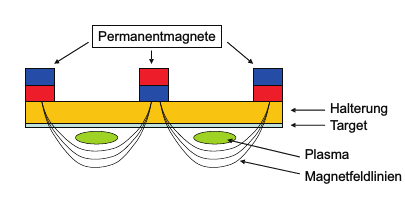
\includegraphics{fig/magneton.png}
    \caption{Schema des Magnetons, welches zum Sputtern verwendet wird
    \cite{fprakt}.}
    \label{fig:magneton}
\end{figure}
Nun muss das Aluminium aufgedampft werden.  Dafür wird das Ag wieder abgesaugt
und der Probenhalter wird um 180$^\circ$ nach unten gedreht. Die Schablone wird
in die nächste Stellung gedreht und das Aluminium wird durch einen Wolframdraht
erhitzt. Wolfram wird deswegen gewählt, weil es eine besonders hohe
Schmelztemperatur besitzt. Es muss zunächst langsam erhitzt werden, da die
Oxidschicht des Aluminiums zuerst weggedampft werden soll. Während dieses
Vorwärmens muss die Schutzblende über der Probe positioniert sein, damit sie kein
Aluminiumoxid abbekommt. Wenn das Aluminium geschmolzen ist, kann die Scheibe
entfernt werden und der Aufdampfvorgang beginnt. Vorher muss die
Schwingungsquarzwaage wissen, dass nun Aluminium verwendet wird.
Die Al-Schichtdicke soll ungefähr bei 50\;nm liegen.
Jetzt kommt der kritischste Punkt des Versuches, nämlich die Herstellung der
Tunnelbarriere. Hierfür wird für eine kurze Zeit eine besonders dosierte Menge
Luft eingelassen, sodass das Aluminium oberflächlich oxidiert. Die genaue
Luftmenge und die Belüftungszeit liegen als Rezept im Labor vor.
Nach der Oxidation wird wieder ein Vakuum erzeugt. Jetzt kann als letzter
Schritt das Blei aufgedampft werden. Dafür wird wieder zunächst die Blende
weiter gedreht und anschließend das Blei verdampft. Es soll eine Schichtdicke
von ca. 300\;nm aufgedampft werden.

Als letztes wird die Probe mithilfe eines Mikroskops untersucht. Hierbei ist
insbesondere darauf zu achten, dass die Kontakte unversehrt sind. In unserem
Fall waren Einkerbungen höchstens so breit wie 1/3 der Kontaktbreite und
sollten somit in Ordnung sein.
\begin{figure}[]
    \centering
    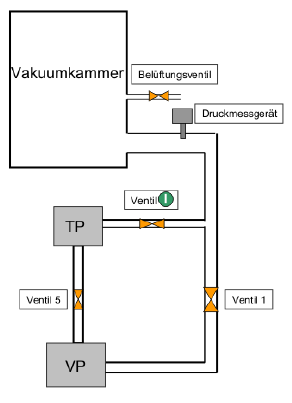
\includegraphics{fig/vakuum.png}
    \caption{Vakuumanlage mit Vorpumpe und Turbopumpe \cite{fprakt}.}
    \label{fig:vakuum}
\end{figure}

\subsection{Einbau der Probe und Messung des Tunnelstroms}
Das Substrat wird zunächst in die Messsonde eingebaut. Dafür werden die sechs
Kontakte mit Indiumplättchen mit der Messsonde verbunden. Indium ist ein
besonders weiches Metall, wodurch ein guter Kontakt mit den Kontakten der Sonde
sichergestellt wird. Jetzt sollten die Kontakte mit einem Amperemeter vermessen
werden. Alle Widerstandswerte unserer Probe waren in diesem Zustand wie zu
erwarten.
Die Messsonde kann jetzt in das Kryostat eingebaut werden. Anschließend wird
die Messung des Tunnelstroms bei Zimmertemperatur durchgeführt. Sowohl Blei als
auch Aluminium sind also Normalleiter. Die Messung geschieht automatisch am
Computer. Hierbei wird eine sogenannte Vierpunktmessung verwendet. Diese
eliminiert den Leitungs- und den Kontaktwiderstand und ist dadurch besonders
geeignet für kleine Tunnelströme.
Mit Origin können die gemessenen Werte direkt angezeigt werden.
Bereits hier hat sich gezeigt, dass unsere Messwerte für die Spannung
ungefähr um 2 Größenordnungen zu hoch sind.
Nun wird das He-Verdampfungskryostat für die SL/NL-Messung vorbereitet. Dazu wird zunächst mit einer Vakuumpumpe das doppelwandige Gefäß evakuiert. Anschließend wird flüssiger
Stickstoff in die Außenwände gefüllt. Dieses kühlt das Gefäß vor und dient als
zusätzlicher Wärmeisolator für das flüssige Helium. Mit dem flüssigen Helium
wird die Probe auf $4.2$\;K heruntergekühlt. Bei dieser Temperatur ist das Blei
bereits supraleitend. Nun wird die erste Tunnelkennlinie
aufgenommen. Auch hier haben unsere Messungen grundsätzlich falsche Ergebnisse
geliefert. Es war keine charakteristische Tunnelkennlinie zu beobachten. \\
Um die Temperaturabhängigkeit der Kennlinien zu untersuchen wird als
letztes der Dampfdruck erniedrigt, wodurch Temperaturen bis zu 1.5\;K erreicht
werden. Hier könnten sich eventuell bereits erste Supraleitende Eigenschaften des
Aluminiums herauszeichnen. Da der Druck kontinuierlich erniedrigt wird, sind
die hier gemessenen Kennlinien in Wahrheit temperaturabhängig. Es wird also ein
Temperatursweep durchgeführt: Kurz vor der gewünschten Temperatur wird die
Messung gestartet. Diese dauert dann 30 Sekunden. Währenddessen sinkt der Druck
weiter. Aus der Dampfdruckkurve von Helium, welche am Kryostat vermerkt ist,
kann dadurch ein Temperaturintervall abgeschätzt werden, welcher als Fehler in
die Auswertung eingeht.

\section{Auswertung}
\label{sec:auswertung}
Da die Daten, welche während unseres eigenen Versuches aufgenommen wurden,
keine sinnvolle Auswertung erlaubten, handelt es sich im folgenden um Altdaten,
die vom Praktikumsassistenten bereitgestellt wurden.
\subsection{NL/NL-Kennlinie bei Raumtemperatur}
\begin{figure}[]
    \centering
    % GNUPLOT: LaTeX picture with Postscript
\begingroup
  \makeatletter
  \providecommand\color[2][]{%
    \GenericError{(gnuplot) \space\space\space\@spaces}{%
      Package color not loaded in conjunction with
      terminal option `colourtext'%
    }{See the gnuplot documentation for explanation.%
    }{Either use 'blacktext' in gnuplot or load the package
      color.sty in LaTeX.}%
    \renewcommand\color[2][]{}%
  }%
  \providecommand\includegraphics[2][]{%
    \GenericError{(gnuplot) \space\space\space\@spaces}{%
      Package graphicx or graphics not loaded%
    }{See the gnuplot documentation for explanation.%
    }{The gnuplot epslatex terminal needs graphicx.sty or graphics.sty.}%
    \renewcommand\includegraphics[2][]{}%
  }%
  \providecommand\rotatebox[2]{#2}%
  \@ifundefined{ifGPcolor}{%
    \newif\ifGPcolor
    \GPcolortrue
  }{}%
  \@ifundefined{ifGPblacktext}{%
    \newif\ifGPblacktext
    \GPblacktexttrue
  }{}%
  % define a \g@addto@macro without @ in the name:
  \let\gplgaddtomacro\g@addto@macro
  % define empty templates for all commands taking text:
  \gdef\gplbacktext{}%
  \gdef\gplfronttext{}%
  \makeatother
  \ifGPblacktext
    % no textcolor at all
    \def\colorrgb#1{}%
    \def\colorgray#1{}%
  \else
    % gray or color?
    \ifGPcolor
      \def\colorrgb#1{\color[rgb]{#1}}%
      \def\colorgray#1{\color[gray]{#1}}%
      \expandafter\def\csname LTw\endcsname{\color{white}}%
      \expandafter\def\csname LTb\endcsname{\color{black}}%
      \expandafter\def\csname LTa\endcsname{\color{black}}%
      \expandafter\def\csname LT0\endcsname{\color[rgb]{1,0,0}}%
      \expandafter\def\csname LT1\endcsname{\color[rgb]{0,1,0}}%
      \expandafter\def\csname LT2\endcsname{\color[rgb]{0,0,1}}%
      \expandafter\def\csname LT3\endcsname{\color[rgb]{1,0,1}}%
      \expandafter\def\csname LT4\endcsname{\color[rgb]{0,1,1}}%
      \expandafter\def\csname LT5\endcsname{\color[rgb]{1,1,0}}%
      \expandafter\def\csname LT6\endcsname{\color[rgb]{0,0,0}}%
      \expandafter\def\csname LT7\endcsname{\color[rgb]{1,0.3,0}}%
      \expandafter\def\csname LT8\endcsname{\color[rgb]{0.5,0.5,0.5}}%
    \else
      % gray
      \def\colorrgb#1{\color{black}}%
      \def\colorgray#1{\color[gray]{#1}}%
      \expandafter\def\csname LTw\endcsname{\color{white}}%
      \expandafter\def\csname LTb\endcsname{\color{black}}%
      \expandafter\def\csname LTa\endcsname{\color{black}}%
      \expandafter\def\csname LT0\endcsname{\color{black}}%
      \expandafter\def\csname LT1\endcsname{\color{black}}%
      \expandafter\def\csname LT2\endcsname{\color{black}}%
      \expandafter\def\csname LT3\endcsname{\color{black}}%
      \expandafter\def\csname LT4\endcsname{\color{black}}%
      \expandafter\def\csname LT5\endcsname{\color{black}}%
      \expandafter\def\csname LT6\endcsname{\color{black}}%
      \expandafter\def\csname LT7\endcsname{\color{black}}%
      \expandafter\def\csname LT8\endcsname{\color{black}}%
    \fi
  \fi
  \setlength{\unitlength}{0.0500bp}%
  \begin{picture}(7200.00,5040.00)%
    \gplgaddtomacro\gplbacktext{%
      \csname LTb\endcsname%
      \put(1342,704){\makebox(0,0)[r]{\strut{}-0.0006}}%
      \put(1342,1383){\makebox(0,0)[r]{\strut{}-0.0004}}%
      \put(1342,2061){\makebox(0,0)[r]{\strut{}-0.0002}}%
      \put(1342,2740){\makebox(0,0)[r]{\strut{} 0}}%
      \put(1342,3418){\makebox(0,0)[r]{\strut{} 0.0002}}%
      \put(1342,4097){\makebox(0,0)[r]{\strut{} 0.0004}}%
      \put(1342,4775){\makebox(0,0)[r]{\strut{} 0.0006}}%
      \put(1474,484){\makebox(0,0){\strut{}-0.008}}%
      \put(2140,484){\makebox(0,0){\strut{}-0.006}}%
      \put(2806,484){\makebox(0,0){\strut{}-0.004}}%
      \put(3472,484){\makebox(0,0){\strut{}-0.002}}%
      \put(4139,484){\makebox(0,0){\strut{} 0}}%
      \put(4805,484){\makebox(0,0){\strut{} 0.002}}%
      \put(5471,484){\makebox(0,0){\strut{} 0.004}}%
      \put(6137,484){\makebox(0,0){\strut{} 0.006}}%
      \put(6803,484){\makebox(0,0){\strut{} 0.008}}%
      \put(176,2739){\rotatebox{-270}{\makebox(0,0){\strut{}Stromstärke I [A]}}}%
      \put(4138,154){\makebox(0,0){\strut{}Spannung U [V]}}%
    }%
    \gplgaddtomacro\gplfronttext{%
      \csname LTb\endcsname%
      \put(5816,4602){\makebox(0,0)[r]{\strut{}Messdaten}}%
      \csname LTb\endcsname%
      \put(5816,4382){\makebox(0,0)[r]{\strut{}fit}}%
    }%
    \gplbacktext
    \put(0,0){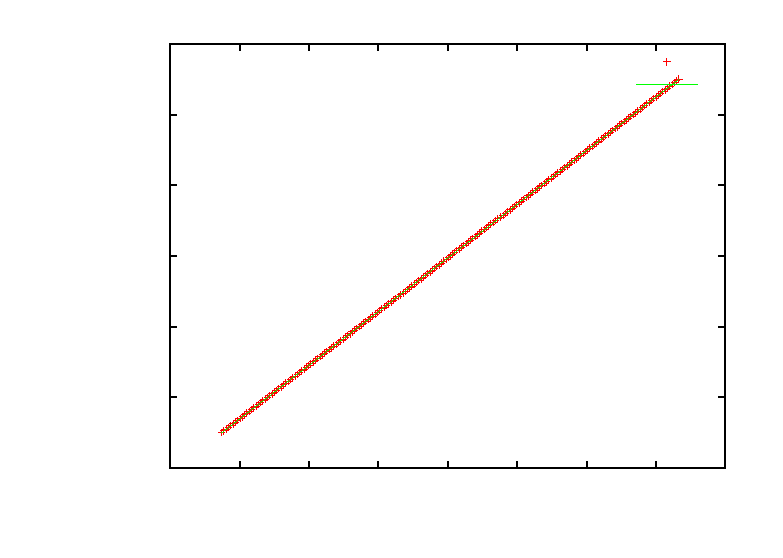
\includegraphics{linfit}}%
    \gplfronttext
  \end{picture}%
\endgroup

    \caption{Bei Raumtemperatur gemessene Strom-Spannungskurve (rot). In grün:
    Linearer fit. Es handelt sich
    um eine Ohm'sche Kennlinie mit konstanter Leitfähigkeit 
    $\sigma=(0.07591\pm0.00001)\;\Omega$.}
    \label{fig:1}
\end{figure}
Für die bei Raumtemperatur gemessene Stromkennlinie erwartet man eine
Proportionalitätsgerade nach dem Ohm'schen Gesetz $I=U/R=\sigma U$, wobei
$\sigma=1/R$ die Leitfähigkeit ist. Um den Widerstand zu
ermitteln, wird also ein linearer fit mit dem Ansatz $f(U)=\sigma U+b$ durchgeführt. Die Ergebnisse sind in Abb.
\ref{fig:1} zu sehen. Für die Fitgrößen ergeben sich:
\begin{align}
    \sigma&=(0.07591\pm0.00001)\;\Omega\\
    b&=(-5.717\times10^{-6}\pm0.03\times10^{-6})\;\text{A}
    \label{eq:linfit}
\end{align}
Hieraus ergibt sich der Widerstand zu $R=(13.173\pm0.002)\;\Omega$, wobei die
Gauß'sche Fehlerfortpflanzungsformel verwendet wurde. Da die Fehler der
Messwerte, welche
symmetrisch sind,
hier keine Auswirkungen auf den fit haben und zudem sehr klein sind
($\sigma_A=0.1$\;mA), wurden sie nicht in die Grafik mit eingetragen.


\subsection{SL/NL-Kennlinien}
\begin{figure}[h]
    \centering
    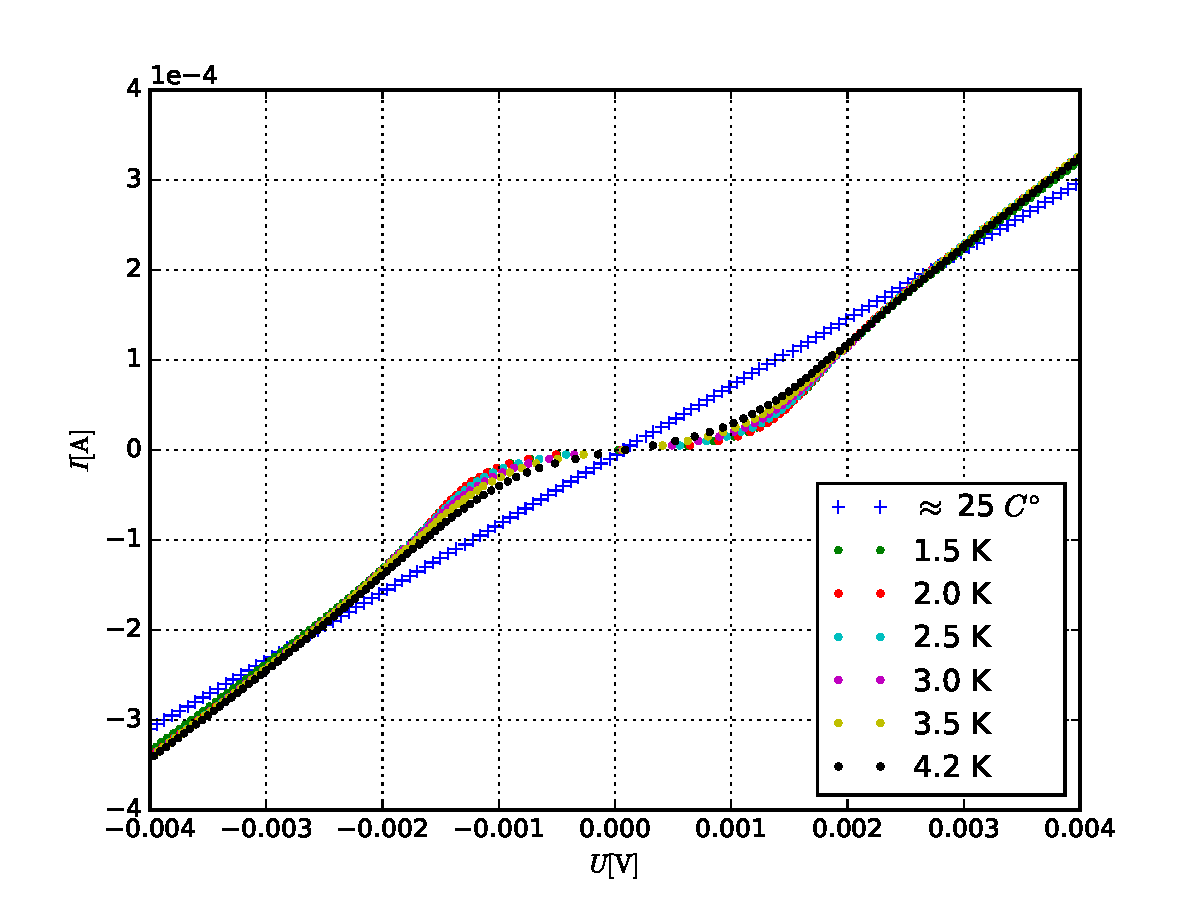
\includegraphics[width=\textwidth]{fig/2.pdf}
    \caption{Gemessene Tunnelkennlinien bei unterschiedlichen Temperaturen.
    Außerdem eingezeichnet ist die Raumtemperaturmessung. Alle qualitativen
    Eigenschaften von Tunnelkennlinien sind wieder zu erkennen. Außerdem laufen
    die Supraleitungs-Kennlinien in etwa gegen die Raumtemperaturmessung.}
    \label{fig:2}
\end{figure}
In Abb. \ref{fig:2} sind die gemessenen Daten von der SL/NL-Messung bei verschiedenen Temperaturen
aufgetragen. Wie bereits erwähnt handelt es sich um einen Temperatursweep um
die gewünschte Temperatur. Es sind deutlich die theoretisch vorhergesagten
Plateaus zu sehen. Bei sehr geringen Spannungen fließt kaum Strom, da die
Energielücke $\Delta$ noch nicht überwunden wurde. Um $\Delta$ zu bestimmen,
werden die Daten numerisch mithilfe des zentralen Differenzenquotienten
\begin{align}
    \diff{I_j}{U}\approx\frac{1}{2}\left(\frac{I_{j+1}-I_j}{U_{j+1}-U_{j}}+\frac{I_{j}-I_{j-1}}{U_{j}-U_{j-1}}\right)
    \label{eq:diffquot}
\end{align}
in einem Python-Skript abgeleitet. Die Ergebnisse hiervon sind in Abb.
\ref{fig:3} zu sehen. Um den Bereich abzuschätzen, ab dem der
Stromfluss beginnt, wird das Maximum der Ableitung gesucht. Dies ist nötig, da
für $T\neq0$ die Kennlinien ``aufgeweicht'' sind und kein klarer Sprung zu
erkennen ist. Als grobe Näherung reicht es jedoch, das Maximum der Ableitung
(= Leitfähigkeit) zu
betrachten, da sich dieses ungefähr an der Stelle des Sprunges bei $T=0$
befindet. Die Ableitung oszilliert sehr stark, eine Interpolation ist demnach
nicht sehr sinnvoll einzusetzen. Für eine grobe Auswertung wird lediglich der
tatsächliche maximale Wert für die Leitfähigkeit genommen und ein großzügiges
Fehlerintervall von $\pm$ 1\;mV abgeschätzt. Eine weitere Möglichkeit wäre es,
das Maximum als Schnittpunkt zweier linearer Fits zu ermitteln, aber aufgrund
der starken Oszillationen wären diese Fits stark abhängig von dem
Fit-Intervall. Es ist also unwahrscheinlich, dass dies zu besseren Ergebnissen
führt. Da die Fehler hauptsächlich von der Position des Maximums abhängen, sind
die Messfehler von $\sigma_I=0.1$\;mA ebenfalls vernachlässigbar. Diese sind
bereits mit dem großzügigen Fehlerintervall für $U$ berücksichtigt. Die Maxima
werden sowohl bei positiven als auch negativen Spannungen gemessen. Dadurch
kann man das doppelte Plateau $2\Delta=U_{\text{max,rechts}}-U_{\text{max,links}}$ bestimmen.
Nach der Gauß'schen Fehlerfortpflanzung ergibt sich
$\sigma_{2\Delta}=\sqrt{\sigma_{\text{max,links}}^2+\sigma_{\text{max,rechts}}^2}=1.4\;\sigma_{\text{max,links}}$.
Die Ergebnisse sind in Tab. \ref{tab:res1} eingetragen.
\begin{table}[!h]
    \centering
    \begin{tabular}{|c|c|c|c|c|}
        \hline
        &\multicolumn{2}{|c|}{Ohne Korrektur}&\multicolumn{2}{|c|}{Mit
        Korrektur}\\\hline
        Temperatur $T [K]$&$2\Delta(T)$
        $[mV]$&$2\Delta(T)/(k_BT_C)$&$2\Delta(T)$
        $[mV]$&$2\Delta(T)/(k_BT_C)$\\\hline
        $1.50\pm0.08$&$3.5\pm1.4$&$5.6\pm2.3$&$1.6\pm1.0$&$5.0\pm3.3$\\\hline
        $2.00\pm0.10$&$3.0\pm1.4$&$4.8\pm2.3$&$1.2\pm1.1$&$3.8\pm3.5$\\\hline
        $2.50\pm0.13$&$3.4\pm1.4$&$5.4\pm2.3$&$1.4\pm1.4$&$4.4\pm3.5$\\\hline
        $3.00\pm0.15$&$4.0\pm1.4$&$6.5\pm2.3$&$1.7\pm1.1$&$5.3\pm3.5$\\\hline
        $3.50\pm0.18$&$3.5\pm1.4$&$5.6\pm2.3$&$1.1\pm1.2$&$3.6\pm4.1$\\\hline
        $4.20\pm0.21$&$3.9\pm1.4$&$6.3\pm2.3$&$0.9\pm1.6$&$2.8\pm5.3$\\\hline\hline
        \multicolumn{4}{|c|}{$\text{Literaturwert: }
        2\Delta_{\text{Pb}}(T=1K)/(k_BT_{C,Pb})$}&$4.33\pm0.10$
        \cite{giaever1961study}\\\hline

    \end{tabular}
    \caption{Ergebnisse für die Energielücke $\Delta$ in mV und in
    dimensionslosen Größen, mit und ohne Korrektur.}
    \label{tab:res1}
\end{table}
\begin{figure}[h]
    \centering
    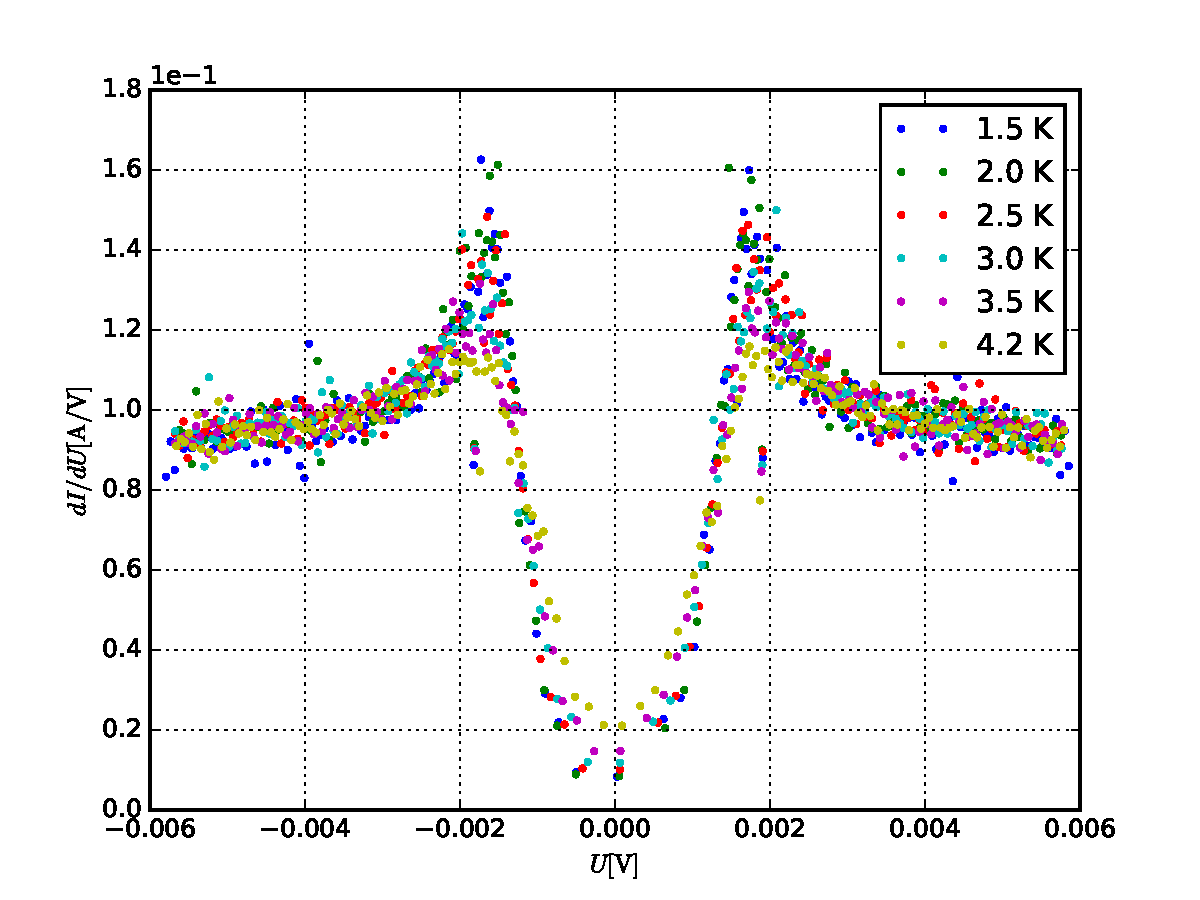
\includegraphics[width=\textwidth]{fig/3.pdf}
    \caption{Ableitung des Tunnelstroms nach der Spannung aufgetragen gegen die
 Spannung. Es sind deutliche Maxima auf beiden Seiten zu sehen. Wie erwartet
 sind diese bei hohen Temperaturen größer. Auf Fehlerbalken wurde zugunsten
 Übersicht verzichtet. }
    \label{fig:3}
\end{figure}
Nach \cite{pike1971} existiert eine Korrekturformel für die Energielücke, die
Quasiteilchenanregungen bei endlicher Temperatur berücksichtigt. Sie lautet:
\begin{align}
    \label{eq:korrektur}
    \Delta_K=\left( \left( eU_{\text{max}}-ak_BT \right)^h-\left( bk_BT
    \right)^h \right)^{\frac{1}{h}}.
\end{align}
Für den Fehler ergibt sich nach Gauß'scher Fehlerfortpflanzung
\begin{align}
    \label{eq:fehlerkorrektur}
    \sigma_{\Delta_{K}}(T)&=\sqrt{(e
    \Delta_{K}(T)^{2h-1}\sigma_{U_{\text{max}}})^2+(ak_BhT^{h-1}
    \Delta_K(T)^{2h-1}\sigma_T)^2}.
\end{align}
Die Parameter sind gegeben durch \cite{pike1971}:
\begin{align}
    a=1.113,\quad b=2.107,\quad h=2.138.
\end{align}
Es ist zu beachten, dass nun eine explizite Temperaturabhängigkeit vorhanden
ist. Der Fehler der Temperatur, die durch den Temperatursweep entstehen, kann
mithilfe der Dampfdruckkurve von Helium abgeschätzt werden. Durch die
exponentielle Abhängigkeit wird der Fehler bei hohen Temperaturen größer.
Allerdings wirkt diesem Effekt entgegen, dass bei niedrigen Drücken der Druck
langsamer verringert wird. Als
grobe Schätzung wird der Fehler linear interpoliert, mit größeren Fehlern für
höhere Temperaturen. Die Ergebnisse sind
in Tab. \ref{tab:res1} zu sehen.
Die kritische Temperatur von Blei ist $T_{C,Pb}=7.2K$ \cite{fprakt}.


\subsection{Vergleich mit der BCS-Theorie}
Mithilfe der BCS-Theorie lässt sich ein Ausdruck für die Energielücke $\Delta$,
die Zustandsdichte $D(E_F)$ bei der Fermienergie sowie die Temperatur $T$
finden. Dies ist ausführlich \zB in \cite{enss2011tieftemperaturphysik}
beschrieben. Man erhält folgende Integraldarstellung:
\begin{align}
    \label{eq:bcsint}
    \frac{2}{D(E_F)\nu_0}=\int_0^{\hbar \omega_D}\frac{\d
    \eta}{\sqrt{\eta^2+\Delta^2}}\left[
    \tanh\left({\frac{\sqrt{\eta^2+\Delta^2}}{2k_BT}}\right) \right].
\end{align}
$\nu_0$ ist dabei ein Parameter der anziehenden Wechselwirkung durch Phononen.
Anstatt diesen Ausdruck numerisch zu Integrieren, wird eine Näherungsformel
verwendet \cite{senapati2011spin}:
\begin{align}
    \label{eq:bcsnäherung}
    \Delta(T)&\approx\Delta_0\tanh\left(k\sqrt{\frac{T_C-T}{T}}\right),\\
    k&\approx1.74.
\end{align}
Eine wichtige Größe für den Vergleich mit realen Supraleitern ist die
Energielücke bei $T=0$: $\Delta_0=1.76k_BT_C$.
Die zuvor errechneten Werte für $\Delta$, sowie die nach Gl.
\ref{eq:bcsnäherung} errechnete Theoriekurve sind in Abb. \ref{fig:4}
aufgetragen. Desweiteren wird der Literaturwert für Blei aus Tab.
\ref{tab:res1} als horizontale Linie eingezeichnet.

\begin{figure}[]
    \centering
    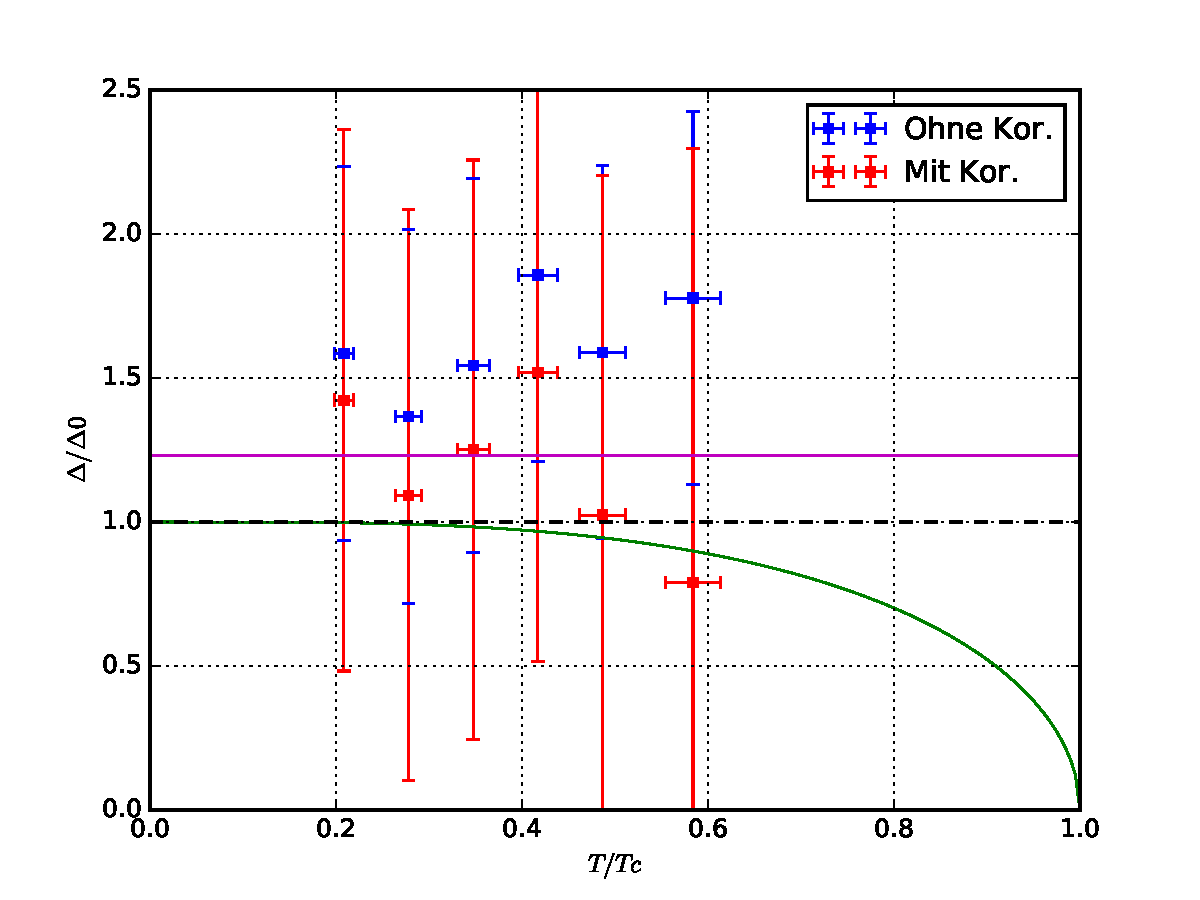
\includegraphics[width=\textwidth]{fig/4.pdf}
    \caption{Unkorrigierte und korrigierte Werte der normierten Energielücke in
    Abhängigkeit von der Temperatur. Außerdem eingezeichnet ist die Vorhersage
    der BCS-Theorie in grün. In Pink ist der Literaturwert für Blei bei 1 Grad
    Kelvin eingezeichnet.}
    \label{fig:4}
\end{figure}
\newpage


\section{Diskussion}
\begin{table}[!h]
    \centering
    \begin{tabular}{|c|c|c|c|c|}
        \hline
        &\multicolumn{2}{|c|}{Ohne Korrektur}&\multicolumn{2}{|c|}{Mit
        Korrektur}\\\hline
        Temperatur $T [K]$&$2\Delta(T)/(k_BT_C)$&$\text{rel. Abw. zum
        Lit. Wert}$&$2\Delta(T)/(k_BT_C)$&$\text{rel. Abw. zum
        Lit. Wert}$\\\hline
        $1.50\pm0.08$&$5.6\pm2.3$&$0.29$&$5.0\pm3.3$&$0.15$\\\hline
        $2.00\pm0.10$&$4.8\pm2.3$&$0.11$&$3.8\pm3.5$&$0.12$\\\hline
        $2.50\pm0.13$&$5.4\pm2.3$&$0.25$&$4.4\pm3.5$&$0.02$\\\hline
        $3.00\pm0.15$&$6.5\pm2.3$&$0.50$&$5.3\pm3.5$&$0.22$\\\hline
        $3.50\pm0.18$&$5.6\pm2.3$&$0.29$&$3.6\pm4.1$&$0.17$\\\hline
        $4.20\pm0.21$&$6.3\pm2.3$&$0.45$&$2.8\pm5.3$&$0.35$\\\hline\hline
        \multicolumn{4}{|c|}{$\text{Literaturwert: }
        2\Delta_{\text{Pb}}(T=1K)/(k_BT_{C,Pb})$}&$4.33\pm0.10$
        \cite{giaever1961study}\\\hline

    \end{tabular}
    \caption{Ergebnisse für die Energielücke $\Delta$ in mV und in
    dimensionslosen Größen, mit und ohne Korrektur, sowie die relative
    Abweichung zum Literaturwert.}
    \label{tab:res2}
\end{table}

\subsection{NL/NL - Messung}
Wie bereits in der Auswertungssektion beschrieben, sind die Daten der
Normalleiter-Normalleiter Kennlinie in sehr guter Übereinstimmung mit der
Theorie. Es zeigt sich deutlich die Ohm'sche Strom-Spannungskurve. Der
errechnete Widerstandswert ist ebenfalls glaubwürdig, da sich die Kennlinien der
SL/NL-Messungen nahezu asymptotisch an NL/NL-Kennlinie anschmiegen. Die hier zu
sehende Diskrepanz ist am wahrscheinlichsten auf die unterschiedliche
Temperatur der beiden Messungen zurückzuführen. So muss bei einem Ohm'schen
Leiter ein Temperaturkoeffizient berücksichtigt werden, der den Widerstand bei
hohen Temperaturen erhöht. Dies ist konsistent zu der kleineren Steigung, also
der geringeren Leitfähigkeit in Abb. \ref{fig:2}, im Vergleich zu den
Supraleitungs-Messungen. 
Da sehr viele Messdaten zu verfügung standen, ist der lineare Fit sehr genau,
was zu einem sehr genauen Ergebnis führt. Dies ist also ein guter Anhaltspunkt
zur qualitativen Überprüfung der SL/NL-Messungen.

\subsection{SL/NL - Messung}
Die in Abb. \ref{fig:2} zu sehenden Kennlinien erfüllen alle qualitativen
theoretischen Vorhersagen. Zum einen erkennt man das charakteristische Plateau
bei geringen Spannungen, bei der kein Tunnelstrom fließt. Desweiteren werden
die Kennlinien aufgeweichter, je höher die Temperatur ist. In Abb.
\ref{fig:3} kann man demnach deutlich erkennen, dass bei niedrigeren
Temperaturen das Maximum der Steigung deutlicher zu erkennen ist. Dieses sollte
theoretisch unendlich sein bei $T=0$. Trotz der höheren maxima bei kleinen
Temperaturen war es schwer, den Punkt des Maximas genau zu bestimmen, aufgrund
der Oszillationen in der numerischen Ableitung. Auch eine zweite numerische
Ableitung hätte demnach nur ein grobes Intervall für den maximalen
Spannungswert geliefert. Es ist möglich, dass eine beidseitige Annährung mit
linearen Fits hier geholfen hätte, obwohl diese - wie bereits erwähnt-
ebenfalls Abhängig von der Fitregion ist. Im Allgemeinen lässt sich sagen, dass
unsere Fehlerabschätzung etwas zu großzügig geworden ist. Dies ist deutlich in
Abb. \ref{fig:4} zu sehen. Die Fehlerbalken sind sowohl bei den korrigierten
Werten, als auch bei den unkorrigierten sehr groß, wobei die
Temperaturabhängigkeit die Fehler der korrigierten Werte nochmals vergrößert.
Der Fehler kommt hier fast ausschließlich durch die Abschätzung des Intervalls
maximaler Spannung. Aufgrund dessen und zugunsten der Übersichtlichkeit wurde auf
Fehlerbalken in den Plots zuvor verzichtet.
Während die Werte ohne Korrektur nicht im ersten Signifikanzintervall die
Literaturkurve der BCS-Theorie schneiden, ist dies für alle korrigierten Werte
der Fall. Aber auch für die korrigierten Werte ist dies nicht unbedingt zu
erwarten, da es sich bei Blei um einen Supraleiter mit starker Phononenkopplung
handelt. Die BCS-Theorie ist aber eine Theorie für geringe Phononenkopplung,
eine Voraussetzung die für Blei nicht gegeben ist. Man muss demnach die
einfache BCS Theorie erweitern, um einen genaueren theoretischen Vergleich mit Blei
herzustellen. Dennoch sind vor allem die korrigierten Werte sehr nahe an der
BCS-Kurve, besonders für hohe Temperaturen. Dies wird bei vielen Versuchen auch
bestätigt \cite{enss2011tieftemperaturphysik}. Die zusätzliche Korrektur zur BCS-Theorie
ist also immer noch relativ gering. Im Vergleich zu dem Literaturwert der dimensionslosen
Energielücke in Tab. \ref{tab:res2} sieht man allgemein, dass die korrigierten
Werte eine mit durchschnittlich 17\% insgesamt niedrigere Abweichung ergeben,
als die unkorrigierten mit einer durchschnittlichen relativen Abweichung von
31\%. Jedoch ist der Theoriewert
bei $T=1$\;K gegeben und man erwartet die beste Übereinstimmung für den
Messwert bei $T=1.5$\;K. Dies ist jedoch hier nicht der Fall. Dennoch schneiden
die Fehlerbalken aller Werte, mit und ohne Korrektur, diesen Theoriewert.
Demnach ist die Messung insgesamt als gelungen einzustufen. Es wurden alle
qualitativen Aussagen der Theorie bestätigt und quantitativ ergeben die Werte,
wenigstens von der Größenordnung her, eine gute Übereinstimmung zur Theorie.





\clearpage

%\appendix
%
%\section{Anhang}
%
%
%\ldots
%
%\clearpage

% nicht unbedingt erforderlich
%\listoffigures
% nicht unbedingt erforderlich
%\listoftables

\bibliography{literatur}

\end{document}

